
\section{Personal Histories}

The following sections will feature many of the same figures;
here we will introduce them so their interleaving stories may be told
uninterrupted in the following sections.
Readers unfamiliar with the history of Unix may find unfamiliar terms in these
personal accounts; these will be discussed in the following sections after
our characters have been introduced.

\subsection{Doug McIlroy, Joined 1958}

Douglas McIlroy was born in Fishkill, New York.
His father worked in electrical engineering and spent time at
MIT and ended his career at Cornel, having contributed to the RADAR effort in World War II.
His father collected maps, and Doug grew an interest in maps himself.
One day, while ill in bed with chicken pox, his father assigned him the task of drawing
a dam on a USGS map, and showing which regions would be inundated by the dam
\cite{doug_mcilroy_oral_history_2019}.
His mother, too, had a master's degree in physics from the University of Rochester,
which was very unusual at the time. She was forced to audit some of her classes there,
because "women can't take this class! But you can sit in on it, if you want."
Thus he was raised in an engineering-minded household.

Barbara, his wife, also studied mathematics and faced discouragement similar to his mother's.
They ended up meeting at the laboratory, where Doug recalled that some figures at the labs sought
to improve the situation for women, specifically Bernie Holbrook.

Doug joined Bell Labs in 1958 and shortly thereafter earned his
PhD in applied mathematics from MIT.
McIlroy became head of the Computing Techniques Research department in 1965, and he's regarded
as one of the most brilliant members of the staff by key members that readers may be more familiar with.

He is described by nearly everyone at the Bell Labs Computing Research Center
(who wrote or spoke about their time there)
as the most brilliant member of that team that no one has heard of
\cite{kernighan_interviews_thompson_2019}; Ken Thompson described him as
"the smartest one of all of us and the least remembered or written down of all of us."

He was relatively hands-off as a manager, preferring to peek into his employees' offices
with suggestions or interesting problems and wait for the employees to let \textit{him} know
what needed to be done, rather than assigning tasks directly.
His employees respected his tasted in technical and personal matters,
as Brian Kernighan describes\cite{kernighan_unix:_2020}:

\begin{quotation}
Unix might not have existed, and certainly
would not have been as successful, without Doug's good taste and sound
judgment of both technical matters and people.
\end{quotation}

\begin{figure}
    \centering
    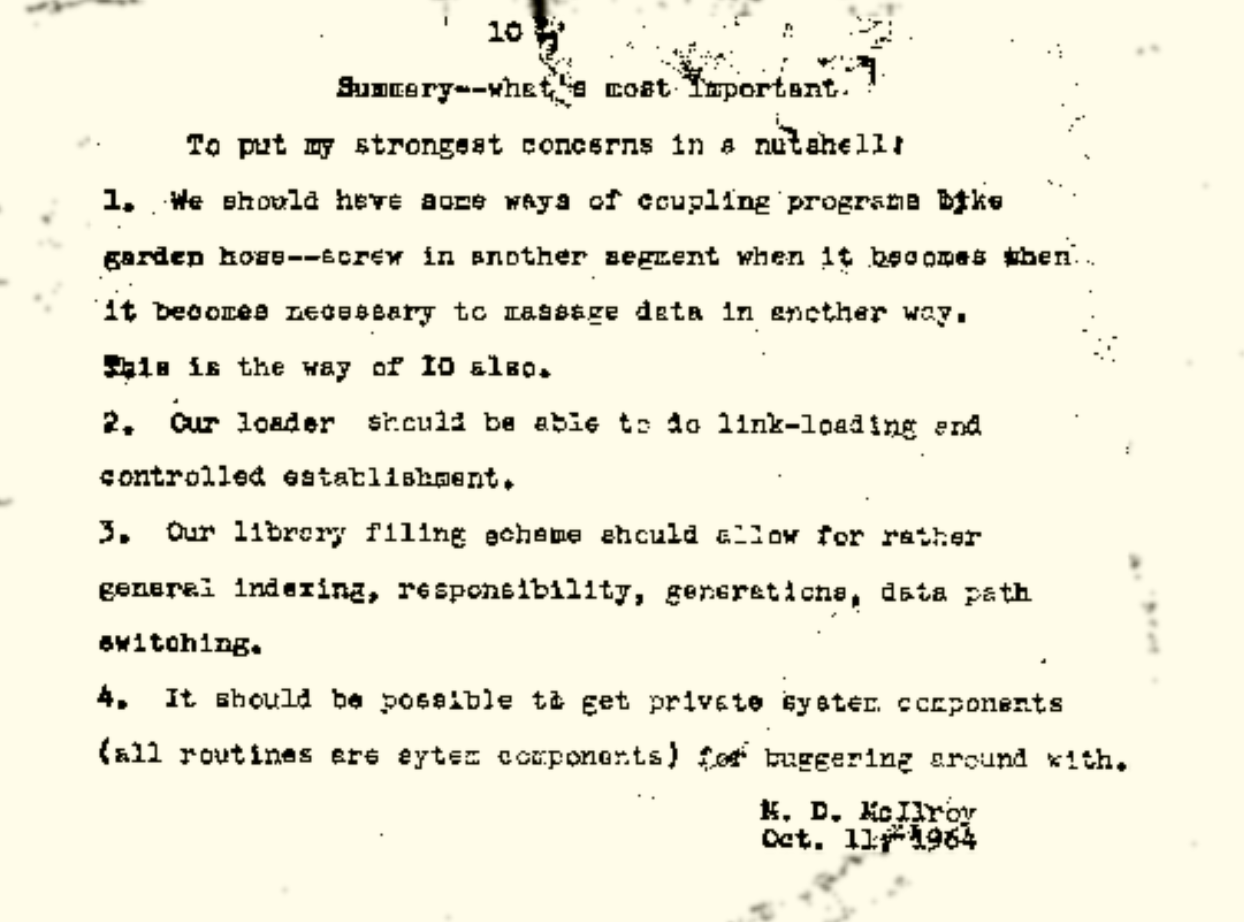
\includegraphics[width=0.7\textwidth]{resource/software/unix/doug-1964-pipes.png}
    \caption{Doug McIlroy's 1964 memo proposing Unix pipes\cite{doug_mcilroy_origin_of_unix_pipes_1964}.}
    \label{fig:unix-pipes-mcilroy-memo}
\end{figure}

In 1964, he circulated a memo which led to Unix pipes\cite{doug_mcilroy_origin_of_unix_pipes_1964}
(see \ref{fig:unix-pipes-mcilroy-memo}) though it took him quite a while to convince
Ken Thompson that he really ought to implement them.
Aside from pipes, he wrote many common Unix utilites we still use today, like
\texttt{diff}, \texttt{sort}, \texttt{join}, \texttt{tr}, \texttt{echo}, \texttt{tee}, and \texttt{spell}.

He hired Alfred Aho in 1967\cite{aho_oral_history_2022}:

\begin{quotation}
I was interviewed by a department head by the name of Doug McIlroy. He was an applied
mathematician from MIT. He had been at Bell Labs for a few years before me. Amongst other things, he
had co-invented macros for programming languages and he's also in this class of one of the smartest
people I've ever met.
\end{quotation}

\subsection{Ken Thompson, Joined 1966}



\subsection{Dennis Ritchie, Joined 1967}



\subsection{Alfred Aho, Joined 1967}

\begin{quotation}
    One of the first people that I met at Princeton was a Columbia graduate by thename of Jeffrey 
Ullman. He had just gotten his undergraduate degree fromColumbia University and also had come to 
study digital systems in the EEdepartment at Princeton. So, he and I became close friends. When we 
graduated from Princeton, we both joined the newly formed Computing Sciences ResearchCenter at Bell 
Labs. There we developed a lifelong collaboration on subjects ranging from algorithms, programming 
languages, to the very foundations of computer science. I was very fortunate to have met some of the 
greatest people in the field and to have gotten to know them and work with them. You learn so much by 
working with the best people in the field. So, I felt very blessed because I had this kind of 
background
\dots
Hsu: Before we jump into Bell Labs more deeply, could you maybe explain-- talk about your PhD 
thesis,but try to explain it to somebody who, maybe like a museum goer who doesn't really know much 
about computer science and linguistics.

Aho: This is interesting. As I mentioned, Hopcroft told me, "Find your own research problem." He 
did teach a course in automata and language theory, so I got introduced to formal language theory 
and automata theory, at least, as it was known at that time. I was interested in programming 
languages and compilers. What I noticed was that a programming language has a syntax and a 
semantics. All languages have a syntax and a semantics. If you want to write a translator for a 
programming language, or even a natural language, you have to understand the syntax and semantics of 
your source language and the target language
\dots

Hansen: 1967, and you followed Ullman there. He had already joined Bell Labs before.

Aho: A few months before me.

Hansen: A few months before. And what group was it that you joined?

Aho: I was interviewed by a department head by the name of Doug McIlroy. He was an 
applied mathematician from MIT. He had been at Bell Labs for a few years before me. Amongst other 
things, he had co invented macros for programming languages and he's also in this class of one of the 
smartest people I've ever met.Jeff wanted to go to academia a little bit earlier than I did, like 
many years earlier. He stayed at Bell Labs for a few years and went to PrincetonUniversity where he 
joined the faculty of the electrical engineering department, but he would come and spend one day a 
week consulting at Bell Labs.His consulting stint was he would come Fridays and sit in my office 
all day.The conversations that we'd have would range over all sorts of topics, and sometimes he'd 
mentioned that he was working on a problem with a colleague atPrinceton, and after describing the 
problem, I might say, "You're kidding," and he said, "Oh, you're right. The solution is obvious, 
isn't it?" I don't know whether I would say dynamic programming or whatever, but several papers 
came out of this intense collaboration, and we got to the point where we could communicate with just 
a few words. We had a very large, shared symbol table.
\cite{aho_oral_history_2022}
\end{quotation}
\begin{quotation}
    But as Unix was being developed, Ken Thompson created the first two versions ofUnix using 
assembly language. He had joined Bell Labs at roughly the same time I had. He was there maybe six 
months or so ahead of us, and he had been assigned to work on the Multics project that BellLabs was 
part of with MIT and GE. When Bell Labs got tired of pouring money into Multics and not getting the 
operating system that it had wanted, it abandoned the project and left Ken Thompson to his 
own devices. Ken thought there were some good ideas in Multics. Being the genius that he was, he 
said, I can do it much more simply and much more elegantly. So he created a rudimentary version of 
Unix and thenkept writing and polishing it. Dennis Ritchie came on the scene. Ken had also created 
a programming language, B. The B was maybe the first letter of BCPL. Who knows? But when Dennis 
Ritchie looked at it, he said, what B needs is a decent type system. So he put a decent type system 
on B, and created theC programming language. Thompson and Ritchie wrote the third version of Unix 
using the newly createdC programming language. I became an early adopter of C, and I had C wired in 
my fingertips, so I could write C programs quite readily, and of course, there were all these neat 
tools that accompanied the programming environment on Unix. There were the text editors. I don't 
know whether you've ever heard of the ED editor or the QED editor that was at MIT as part of 
Multics. QED had regular expressions in it. This triggered my interest in regular expressions. Ken 
Thompson had written a program called grep for doing pattern matching on text files, and it had a 
very limited form of regular expressions when I encountered it.
\cite{aho_oral_history_2022}
\end{quotation}
\begin{quotation}
\textbf{Collaboration with Ullman}

Aho is best known for the textbooks he wrote with Ullman, his co-awardee. 
The two were full time colleagues for three years at Bell Labs, but after 
going back to Princeton as a faculty member Ullman continued to work one day a 
week for Bell.They retained an interest in the intersection of automata theory 
with formal language. In an early paper, Aho and Ullman showed how it was 
possible to makeKnuth's LR(k) parsing algorithm work with simple grammars that 
technically did not meet the requirements of an LR(k) grammar. This technique 
was vital to theUnix software tools developed by Aho and his colleagues at Bell 
Labs. That was just one of many contributions Aho and Ullman made to formal 
language theory and to the invention of efficient algorithms for lexical 
analysis, syntax analysis, code generation, and code optimization. They 
developed efficient algorithms for data-flow analysis that exploited the 
structure of "gotoless" programs, which were at the time just becoming the norm.
\cite{aho_turing_award_2020}
\end{quotation}
\begin{quotation}
\textbf{The Early History of Software, 1952-1968 101}

In the early 1960s computer science struggled to define itself and its 
purpose,in relation not only to established disciplines of electrical 
engineering and applied mathematics, but also in relation to—and as something 
distinct from—the use of computers on campus to do accounting, record keeping, 
and administrative work.58 Among those responsible for the discipline that 
emerged, Professor George Forsythe of Stanford's mathematics faculty was 
probably the most influential. With his prodding, a Division of Computer Science 
opened in the mathematics department in 1961; in 1965 Stanford established a 
separate department, one of the first in the country and still one of the 
most well-regarded.59
\cite{history_of_modern_computing_2003_ceruzzi}
\end{quotation}
\todo{Dragon book; all the books Aho, Ullman and others worked on together.}
\section{Compiler-Compilers}
\todo{Yacc and Lex made with Aho's help. then everyone started making mini languages.AWK. 
"Kernighan and Cherry developed a little language for specifyingmathematics called EQN using these 
tools"}
\begin{quotation}
    People started using the Kernighan and Lorinda Cherry EQN tool to specify mathematics in their 
documents and in the research papers that they were writing. They would feed the EQN specification 
into the typesetting program roff
\dots
Knuth adopted the EQN language to include in the TeX typesetting system, and in LaTeX. It's 
basically Kernighan and Cherry's way of specifying mathematics. These software tools had a great 
deal of influence, and Kernighan and Cherry enjoyed the fruits of parsing theory and formal language 
theory in using the tools Lex and Yacc to create their EQN typesetting language. Knuth has this 
saying that the best theory is motivated by practice and the best practice by theory. I internalized 
that with my early experience in the Computing SciencesResearch Center because I found that the 
theory that we were developing in computer science could be applied to document preparation systems, 
programming languages, compilers, and so on. It was really avery productive environment. I taught 
courses on compiler design at local universities, and then when I went to Columbia, I would teach 
the course on programming languages and their translators
\dots
I might point out that the first Fortran compiler developed by IBM in the 1950s took 18 staff years 
to create. In my programming languages and compilers course, I organized the students into teams of 
four or five. Each team had to create their own programming language, and then write a translator 
for it, and in all the time that I taught the course for almost 25 years at Columbia to thousands of 
students, never did a team failed to deliver a working compiler in the 15-week course, and I 
attribute that to the abstractions
\cite{aho_oral_history_2022}
\end{quotation}
\begin{quotation}
    Aho: Okay. AWK is a programming language that was created by me, Brian 
Kernighan, and Peter Weinberger.

Hsu: And it's your three initials that are in.

Aho: Yes. I'm the A in AWK. Weinberger is the W in AWK and Kernighan is the 
K in AWK.We thought that it was just a throwaway tool for us, nobody really 
would be interested in it. But it's amazing how much routine data processing 
there is in the world.The reason the language got to be known as AWK was because 
when our colleagues would see the three of us in one office or another, and when 
they'd walk past the open door, they'd say, AWK, AWK, AWK as they were going 
down the corridor. So we had no choice but to call it AWK because of the 
good-natured ribbing we got from our colleagues, and because at some Unix 
conference, they passed out t-shirts that had AWK,and the error message saying 
"bailing out on or near line five" on them.
\end{quotation}

\subsection{Jeffrey Ullman, Joined 1967}



\subsection{Brian Kernighan, Joined 1969}
